\documentclass{uimppracticas}

%Permitir cabeceras y pie de páginas personalizados
\pagestyle{fancy}

%Path por defecto de las imágenes
\graphicspath{ {./images/} }

%Declarar formato de encabezado y pie de página de las páginas del documento
\fancypagestyle{doc}{
  %Pie de Página
  \footerpr{}{}{{\thepage} de \pageref{LastPage}}
}

%Declarar formato de encabezado y pie del título e indice
\fancypagestyle{titu}{%
  %Cabecera
  \headerpr{}{}{}
  %Pie de Página
  \footerpr{}{}{}
}

\appto\frontmatter{\pagestyle{titu}}
\appto\mainmatter{\pagestyle{doc}}

\begin{document}
	
%Comienzo formato título
\frontmatter

%Portada (Centrado todo)
\centeredtitle{./images/LogoUIMP.png}{Máster Universitario en Investigación en Inteligencia Artificial}{Curso 2020-2021}{Recuperación y extracción de información, \\ grafos y redes sociales}{Práctica Bloque II: Recuperación de información y minería de texto}

\begin{center}
\large \today
\end{center}

\vspace{40mm}

\begin{flushright}
 	{\bf Laura Rodríguez Navas}\\
 	\textbf{DNI:} 43630508Z\\
 	\textbf{e-mail:} \href{rodrigueznavas@posgrado.uimp.es}{rodrigueznavas@posgrado.uimp.es}
\end{flushright}

\newpage

%Índice
\tableofcontents

\newpage

%Comienzo formato documento general
\mainmatter

\setlength\parskip{2.5ex}

\section{Resumen}

En esta práctica se ha implementado un rastreador web (crawler) en Python~\cite{GitHubRepo} (ver sección~\ref{crawler}), que se complementa con un proceso de agrupamiento, también implementado en Python, de la información extraída de las páginas web que ha recopilado (ver sección~\ref{kmeans}). 

\section{Rastreador web (crawler)}\label{crawler}

En esta sección se describe como se ha implementado el rastreador web (crawler) en Python usando la librería \href{https://scrapy.org/}{Scrapy}. Para empezar con la implementación se debe ejecutar el siguiente comando:

\begin{lstlisting}[language=bash]
$ scrapy startproject books
\end{lstlisting}

Este comando crea un proyecto Scrapy en el directorio books, siguiendo la \href{https://docs.scrapy.org/en/latest/topics/commands.html#default-structure-of-scrapy-projects}{estructura por defecto} común para todos los proyectos Scrapy, y el fichero \textit{scrapy.cfg} que contiene el nombre del módulo de Python que define la configuración del proyecto books (\textit{books.settings}). El proyecto lo he nombrado books, porqué se rastreará el catálogo de libros que se encuentra en la página web: \url{http://books.toscrape.com}.

Una vez se ha creado el proyecto, se definen los ítems de cada libro que se quieren extraer del catálogo. En este caso los ítems que se van a extraer son: el título, la categoría, la descripción, el precio y la valoración de cada libro. Para ello, se tiene que modificar el fichero \textit{books/items.py}, para incluir los cinco ítems que se quieren extraer. Vemos el contenido de \textit{items.py} a continuación:

\begin{lstlisting}[language=python]
import scrapy


class BooksItem(scrapy.Item):
	# define the fields for your item here like:
	# name = scrapy.Field()
	title = scrapy.Field()
	category = scrapy.Field()
	description = scrapy.Field()
	price = scrapy.Field()
	rating = scrapy.Field()
\end{lstlisting}

El siguiente paso es describir la manera de extraer la información definida en el fichero \textit{items.py}. Para ello, se utilizarán reglas de expresión \href{https://www.w3.org/TR/xpath/all/}{XPath} y \href{https://www.w3.org/TR/selectors/}{CSS}. Por ejemplo, si nos fijamos en el código HTML de uno de los libros que se van rastrear (ver Figura \ref{book}), veremos que el título del libro es fácil de extraer con la siguiente regla de expresión CSS: \textbf{"h1 ::text"}. Cuando la extracción de información se complica un poco más, se usan reglas de expresión XPath. Por ejemplo, para extraer las descripciones de todos los libros se usará la regla de expresión: \textbf{"//div[@id='product\_description']/following-sibling::p/text()"}. Una vez, definidas todas las reglas de expresión para cada ítem que se va a rastrear, se crea la araña \textit{books/spiders/books\_toscrape.py}.

Las arañas son clases que definen cómo se rastrea una página web determinada (o un grupo de páginas web), incluido cómo realizar el rastreo y cómo extraer la información deseada. En otras palabras, las arañas son el lugar donde se define el comportamiento personalizado para rastrear y analizar las páginas web. En el caso de la práctica, en la araña \textit{books.toscrape} será el lugar donde se definen las reglas de expresión. En las arañas también se tienen que especificar las solicitudes iniciales para rastrear las URLs y una función de devolución de llamada (\textit{parse}) a la que se llamará para generar los ítems de respuesta de esas solicitudes. Por último, los ítems devueltos por las arañas normalmente se conservan en una base de datos o se escriben en un archivo. En el caso de la práctica, en la araña \textit{books.toscrape}, los ítems (título, categoría, descripción, precio y valoración de cada libro) serán guardados en el fichero \textit{books.json}. Esta araña que procesa todas las URLs descubiertas de la \href{http://books.toscrape.com}{práctica} utilizando la función \textit{parse}, que a su vez llama a la función \textit{parse\_book\_page} donde son definidas todas las reglas de expresión de cómo extraer la información deseada, se muestra a continuación:

\begin{lstlisting}[language=python]
import scrapy


class BooksToscrapeSpider(scrapy.Spider):
	name = 'books.toscrape'
	allowed_domains = ['books.toscrape.com']
	start_urls = ['http://books.toscrape.com/']
	
	def parse(self, response):
		for book_url in response.css("article.product_pod > h3 > a ::attr(href)").extract():
			yield scrapy.Request(response.urljoin(book_url), callback=self.parse_book_page)
		next_page = response.css("li.next > a ::attr(href)").extract_first()
		if next_page:
			yield scrapy.Request(response.urljoin(next_page), callback=self.parse)
	
	@staticmethod
	def parse_book_page(response):
		item = {}
		product = response.css("div.product_main")
		item["title"] = product.css("h1 ::text").extract_first()
		item['category'] = response.xpath("//ul[@class='breadcrumb']/li[@class='active']/preceding-sibling::li[1]/a/text()").extract_first()
		item['description'] = response.xpath("//div[@id='product_description']/following-sibling::p/text()").extract_first()
		price = response.xpath('//th[text()="Price (incl. tax)"]/following-sibling::td/text()').extract_first()
		item['price'] = price.replace('£', '')
		rating = response.xpath('//*[contains(@class, "star-rating")]/@class').extract_first()
		item['rating'] = rating.replace('star-rating ', '')
		yield item
\end{lstlisting}

En este momento ya se puede iniciar la araña, pero primero es recomendable modificar el fichero \textit{books/settings.py} para limitar el acceso de la araña al catálogo web, ya que podemos generar un ataque \href{https://es.wikipedia.org/wiki/Ataque_de_denegaci%C3%B3n_de_servicio}{DDoS}. Para ello, debemos descomentar la variable \href{https://docs.scrapy.org/en/latest/topics/settings.html#download-delay}{DOWNLOAD\_DELAY} y darle un valor en segundos (p.ej. DOWNLOAD\_DELAY = 3). 	
	
\begin{figure}[h]
	\centering
	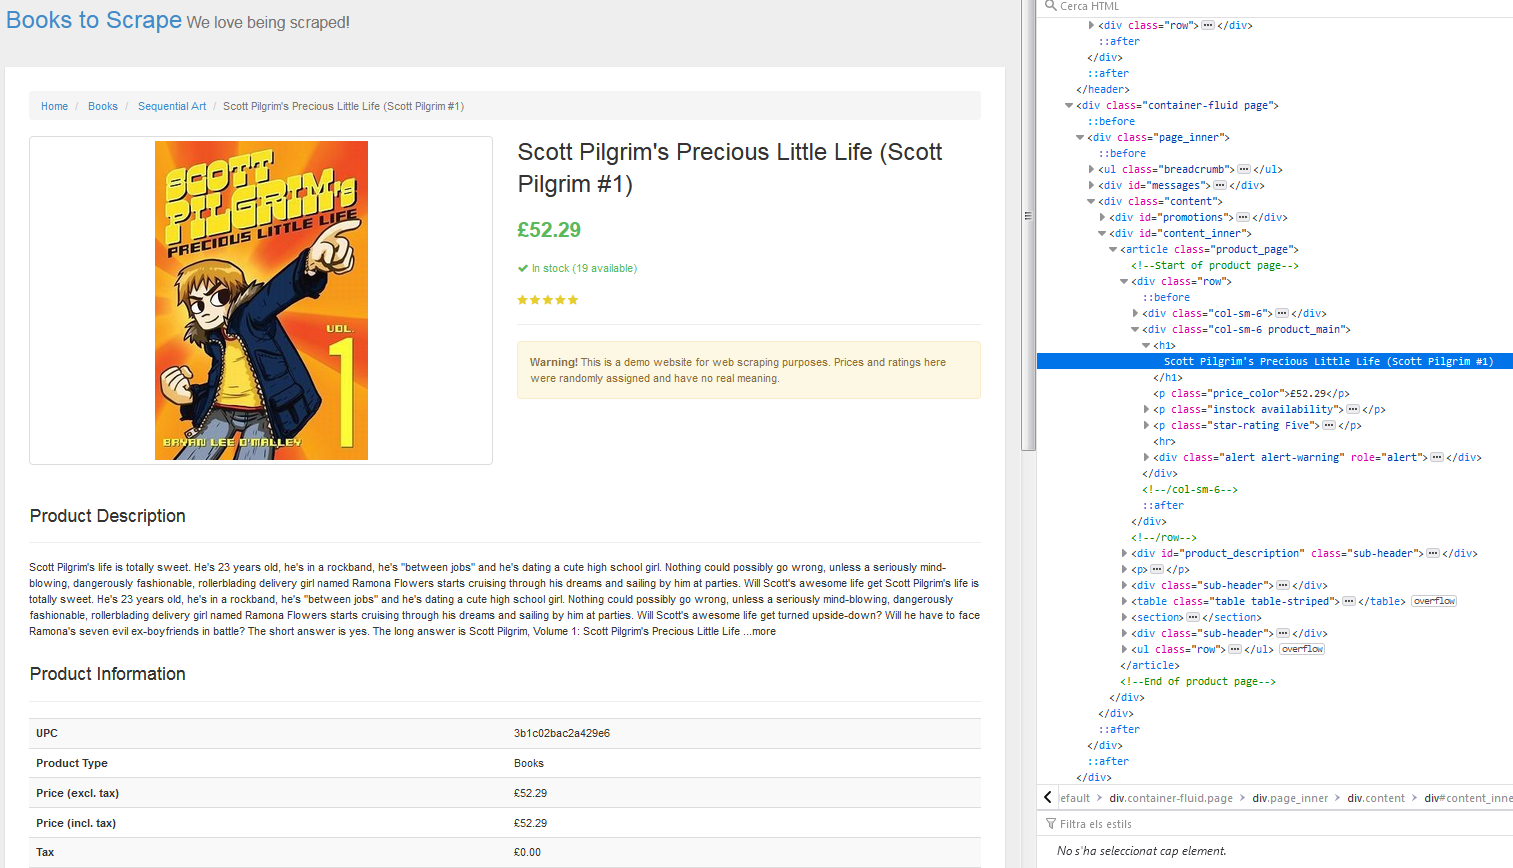
\includegraphics[scale=0.35]{images/book}
	\caption{Ejemplo de libro a rastrear.}
	\label{book}
\end{figure}

Finalmente, ya podemos iniciar la araña para que recupere la información del catálogo y la guarde en el fichero \textit{books.json}:

\begin{lstlisting}[language=bash]
	$ cd books
	$ scrapy crawl books.toscrape -o books.json
\end{lstlisting}

\section{K-Means}\label{kmeans} 

En esta sección se describe como se ha implementado el proceso de agrupamiento en Python (ver directorio kmeans en~\cite{GitHubRepo}) usando la librería scikit-learn~\cite{scikit-learn}. Existen muchos algoritmos de agrupación, y para esta práctica se ha elegido el algoritmo \href{https://scikit-learn.org/stable/modules/generated/sklearn.cluster.KMeans.html}{K-Means}. Concretamente, el algoritmo K-Means agrupará los títulos de los libros del catálogo web (recuperados en la sección~\ref{crawler}) en diferentes clústeres por sus similitudes.

\subsection{Datos de entrada}

Si nos fijamos en \textit{main} del fichero \textit{kmeans/kmeans.py}, vemos que empieza extrayendo la información de los libros almacenada en el fichero \textit{books/books.json} (1000 documentos) y la convierte en un \textit{DataFrame} (ver Definición~\ref{dataframe}). A continuación, se eliminan los valores NaN que pudieran existir en él y es almacenado en un fichero CSV (\textit{kmeans/books.csv}). Para ello, se usa la librería pandas~\cite{jeff_reback_2020_4309786}.

Las primeras líneas del \textit{DataFrame} que forman los datos de entrada:

\begin{table}[h]
	\begin{adjustbox}{width=\columnwidth,center}
		\begin{tabular}{lllll}
			\toprule
			title & category & description & price & rating \\
			\midrule
			Sapiens: A Brief History of Humankind & History & From a renowned historian... & 54.23 & Five \\
			Sharp Objects & Mystery & WICKED above her hipbone, GIRL... & 47.82 & Four \\
			Soumission & Fiction & Dans une France assez... & 50.10 & One \\
			Tipping the Velvet & Historical Fiction & Erotic and absorbing... & 53.74 & One \\
			A Light in the Attic & Poetry & It's hard to imagine... & 51.77 & Three \\
			\bottomrule
		\end{tabular}
	\end{adjustbox}
	\caption{Conjunto de datos de entrada.}
	\label{table1}
\end{table}

En este punto, concretamos la estructura de datos que se utilizará para alimentar el algoritmo K-Means. Se crea una lista que contiene los títulos de los libros.

\begin{lstlisting}[language=python]
titles = df["title"].to_list()
print(titles[:10])  # first 10 titles
>> ['Sapiens: A Brief History of Humankind', 'Sharp Objects', 'Soumission', 'Tipping the Velvet', 'A Light in the Attic', "It's Only the Himalayas", 'Libertarianism for Beginners', 'Mesaerion: The Best Science Fiction Stories 1800-1849', 'Olio', 'Our Band Could Be Your Life: Scenes from the American Indie Underground, 1981-1991']
\end{lstlisting}

\begin{definition}\label{dataframe}
Un DataFrame es una estructura de datos bidimensional etiquetada que acepta diferentes tipos datos de entrada organizados en columnas. Se puede pensar en un DataFrame como una hoja de cálculo o una tabla SQL.
\end{definition}

\subsection{Palabras vacías, derivación y tokenización}

Esta sección se centra en definir algunas funciones para manipular los títulos. Primero, se obtiene la lista de palabras vacías en inglés (ver Definición~\ref{palabras_vacías}), usando la librería NLTK~\cite{bird2009natural}. La lista de palabras vacías es en inglés ya que los títulos de los libros están inglés. Segundo, se obtiene el \textit{Snowball Stemmer}, también usando la librería NLTK, para descomponer las palabras que componen cada título en su raíz.

\begin{lstlisting}[language=python]
# nltk's English stopwords as variable called 'stopwords'	
stopwords = nltk.corpus.stopwords.words('english')  
# nltk's SnowballStemmer as variabled 'stemmer'
stemmer = SnowballStemmer("english")
print(stopwords[:10])   # first 10 stopwords
>> ['i', 'me', 'my', 'myself', 'we', 'our', 'ours', 'ourselves', 'you', "you're"]    
\end{lstlisting}

\begin{definition}\label{palabras_vacías}
	Las palabras vacías son palabras sin significado como artículos, pronombres, preposiciones, etc. que son filtradas antes o después del procesamiento de datos en lenguaje natural (texto).
\end{definition}

A continuación se define la función \textit{tokenize\_and\_stem}: 

\begin{lstlisting}[language=python]
def tokenize_and_stem(text):
	# first tokenize by sentence, then by word to ensure that punctuation is caught as it's own token
	tokens = [word for sent in nltk.sent_tokenize(text) for word in nltk.word_tokenize(sent)]
	filtered_tokens = []
	# filter out any tokens not containing letters (e.g., numeric tokens, raw punctuation)
	for token in tokens:
		if re.search('[a-zA-Z]', token):
			filtered_tokens.append(token)
	stems = [stemmer.stem(t) for t in filtered_tokens]
	return stems  
\end{lstlisting}

Esta función, que divide los títulos en una lista de tokens y los descompone con su raíz, será usada en la siguiente sección para calcular la matriz tf-idf.
 
\subsection{Extracción de características}

\begin{wrapfigure}{r}{0.4\textwidth}
	\centering
	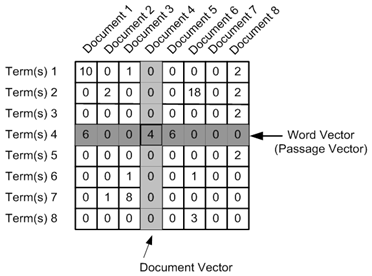
\includegraphics[width=0.4\textwidth]{images/matrix}
	\caption{Matriz \\ de documentos y términos.}
	\label{matrix}
\end{wrapfigure}

En esta sección, se calcula la matriz \href{https://es.wikipedia.org/wiki/Tf-idf}{tf-idf}. Para ello, primero se tienen que contar las apariciones de las palabras por cada documento, que se transforman después en la matriz de documentos y términos (ver Figura~\ref{matrix}). Después, las palabras que aparecen con frecuencia dentro de un documento pero no con frecuencia dentro del \textbf{corpus} reciben una ponderación más alta, ya que se supone que estas palabras contienen más significado en relación con el documento.

\begin{definition}\label{corpus}
En lingüística, un corpus o corpus de texto es un recurso lingüístico formado por un conjunto grande de textos y estructurados.
\end{definition}


La matriz tf-idf para todos los títulos se calcula usando la librería \href{https://scikit-learn.org/stable/modules/generated/sklearn.feature_extraction.text.TfidfVectorizer.html}{sklearn.feature\_extraction.text.TfidfVectorizer}. 

Un par de cosas a tener en cuenta sobre los parámetros definidos en la función TfidfVectorizer son:

\begin{itemize}
	\item max\_features: construye un vocabulario que solo considera las características máximas principales ordenadas por frecuencia de términos de todo el corpus (ver Definición~\ref{corpus}).
	\item use\_idf: habilita la reponderación de frecuencia de documentos inversa.
	\item ngram\_range: define el límite inferior y superior del rango de n-valores para diferentes n-gramos que se extraerán. Principalmente se usa para observar unigramas, bigramas y trigramas. Ver \href{https://en.wikipedia.org/wiki/N-gram}{n-grams}.
\end{itemize}

\begin{lstlisting}[language=python]
# define vectorizer parameters
tfidf_vectorizer = TfidfVectorizer(max_features=200000, stop_words=stopwords, use_idf=True,
	tokenizer=tokenize_and_stem, ngram_range=(1, 3))
tfidf_matrix = tfidf_vectorizer.fit_transform(titles)  # fit the vectorizer to titles
print(tfidf_matrix.shape)
>> (998, 7258)
\end{lstlisting}

Vemos que la matriz tf-idf está formada por 998 documentos y 7258 términos.

\subsection{Entrenamiento del algoritmo}

Ahora pasemos a la parte divertida. Usando la matriz tf-idf, calculada en la sección anterior, se entrena el algoritmo K-Means utilizando \href{https://scikit-learn.org/stable/modules/generated/sklearn.cluster.KMeans.html}{sklearn.cluster.KMeans}. K-means se inicializa con un número predeterminado de clústeres. Elegí 40 como número predeterminado de clústeres, ya que el conjunto de datos contiene libros que pertenecen a una de las 40 categorías, descartando 10 categorías que solo hacen referencia a un único libro.

\begin{lstlisting}[language=python]
# K-Means clustering
num_clusters = 40
km = KMeans(n_clusters=num_clusters)
km.fit(tfidf_matrix)
clusters = km.labels_.tolist()
\end{lstlisting}

Para analizar los resultados del algoritmo, primero creamos un nuevo \textit{Dataframe} con los títulos y su clústeres asignados. Vemos las primeras líneas del contenido del nuevo \textit{Dataframe} a continuación:

\begin{table}[h]
	\centering
	\begin{tabular}{cr}
		\toprule
		title &  cluster \\
		\midrule
		Sapiens: A Brief History of Humankind & 26 \\
		Sharp Objects & 0 \\
		Soumission & 12 \\
		Tipping the Velvet & 12 \\
		A Light in the Attic & 9 \\
		\bottomrule
	\end{tabular}
	\caption{Dataframe de los títulos \\ y su clústeres asignados.}
	\label{table2}
\end{table}


\subsection{Evaluación}


Para la visualización de los clústeres creados en la sección anterior, se tienen que hacer algún prprocesamiento.
\renewcommand{\refname}{Bibliografía}
\bibliographystyle{unsrt}
\bibliography{biblio}

\end{document}
